\section{Diseño preliminar de Comunicaciones Industriales}
%\begin{orientacion}
%El PLC será el nodo principal de control y adquisición. Justifique la arquitectura, los medios y el protocolo con base en el hardware y software disponibles. Separe el control local de la capa IoT; el PLC no debe exponerse directamente a Internet.
%\end{orientacion}

\subsection{Topología y flujo de información}
\begin{figure}[H] 
\centering 
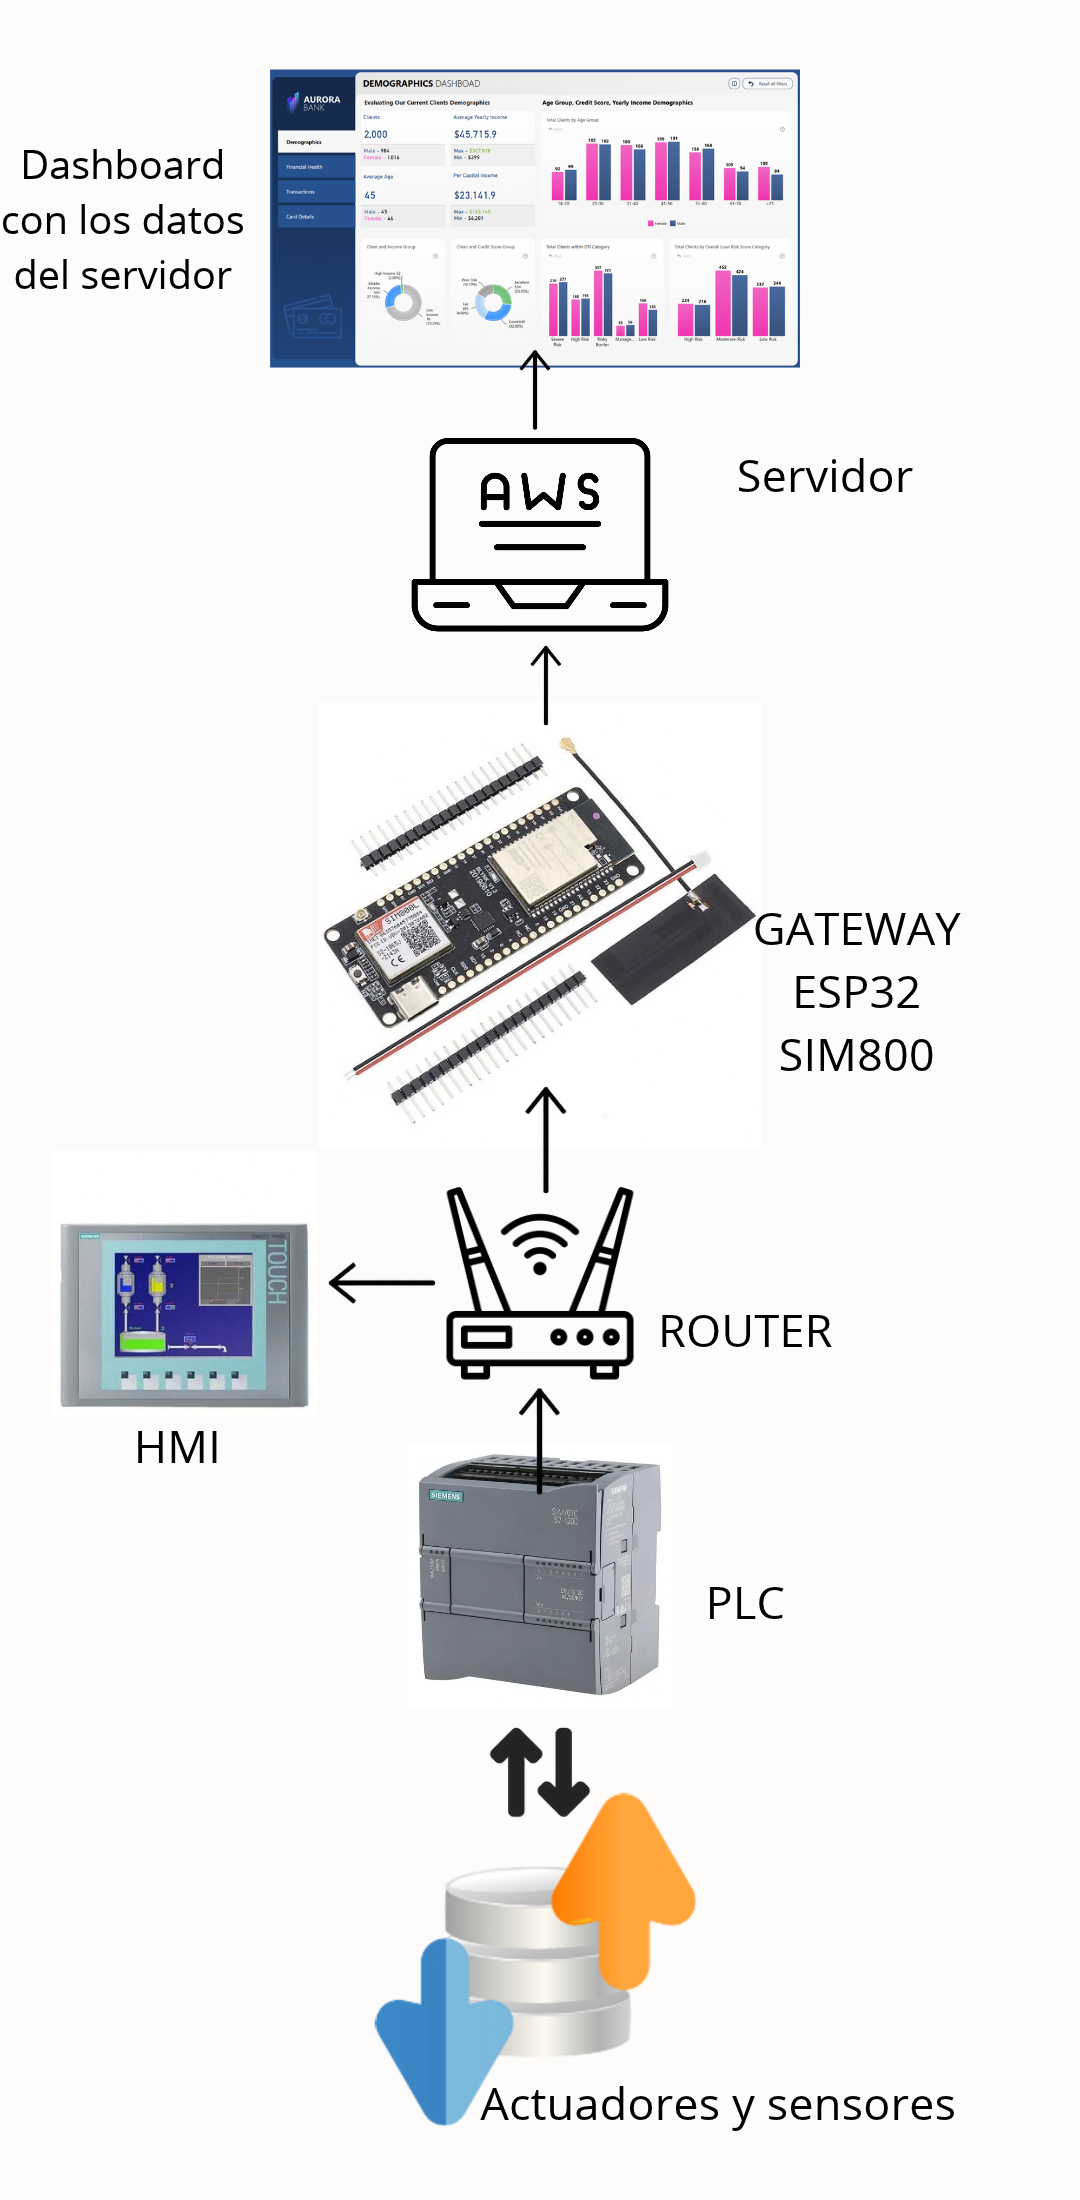
\includegraphics[width=0.5\textwidth]{figuras/Topologia_y_flujo_de_informacion.png} 
\caption{Arquitectura de comunicaciones propuesta.} 
\label{fig:comunicaciones} 
\end{figure} 

{La Figura~\ref{fig:comunicaciones} muestra la arquitectura de comunicaciones implementada, la cual presenta una topología física en estrella dentro de una estructura jerárquica de comunicación. En esta disposición, el router actúa como punto central de interconexión entre el PLC, la HMI y el Gateway ESP32, mientras que el PLC se encarga directamente de la adquisición de datos provenientes de los sensores y del control de los actuadores. Por su parte, el Gateway permite la transferencia de los datos provenientes del sistema de control hacia el servidor, donde estos pueden ser almacenados y visualizados gráficamente como parte del segmento IoT. Los medios físicos utilizados para el intercambio de datos corresponden a Ethernet industrial, empleando el protocolo PROFINET para la comunicación entre los dispositivos de control y visualización compatibles. La disposición propuesta permite mantener al PLC como elemento principal para el control y procesamiento de las variables del proceso, mientras que el Gateway funciona como una interfaz de comunicación entre la red de control y los servicios externos. De esta manera, se evita establecer una conexión directa entre el PLC e Internet, manteniendo separadas las funciones de control industrial y comunicación con la nube. Esta separación contribuye a mejorar la seguridad de la arquitectura de comunicaciones, aspecto relevante en sistemas industriales conectados, debido a los riesgos asociados con la exposición directa de los dispositivos de control a redes externas, como se menciona en Hajda, Jakuszewski y Ogonowski \cite{hajda2021security}.

\subsection{Equipos y direccionamiento IP}
\begin{table}[H]\centering\small\caption{Nodos y direccionamiento IP preliminar.}
\begin{tabularx}{\textwidth}{L{2.8cm}L{2.7cm}L{2.7cm}YL{2.3cm}}\toprule
\textbf{Nodo}&\textbf{IP}&\textbf{Máscara}&\textbf{Función}&\textbf{Interfaz}\\\midrule
PLC&\campo{192.168.x.x}&\campo{255.255.255.0}&Control y adquisición&Ethernet\\
HMI&\campo{192.168.x.x}&\campo{--}&Supervisión local&Ethernet\\
Computador&\campo{192.168.x.x}&\campo{--}&Registro e integración&Ethernet\\\bottomrule
\end{tabularx}\end{table}

{Esta información fue suministrada por el área de comunicaciones de la institución, y se utilizó para la configuración de los equipos de control y visualización. Son accesibles desde el software de programación del PLC (TIA PORTAL), tal como se puede observar en el Anexo G, H e I, donde se muestran las direcciones IP de cada uno de los equipos.}

\subsection{Selección del protocolo}
\begin{table}[H]\centering\scriptsize\caption{Comparación preliminar de protocolos.}
\begin{tabularx}{\textwidth}{L{2.2cm}ccccY}\toprule
\textbf{Protocolo}&\textbf{PLC}&\textbf{HMI}&\textbf{Software}&\textbf{Licencia}&\textbf{Observaciones}\\\midrule
S7&\campo{Sí/No}&\campo{Sí/No}&\campo{--}&\campo{--}&\campo{--}\\
PROFINET&\campo{Sí/No}&\campo{Sí/No}&\campo{--}&\campo{--}&\campo{--}\\
Modbus TCP&\campo{Sí/No}&\campo{Sí/No}&\campo{--}&\campo{--}&\campo{--}\\
OPC UA&\campo{Sí/No}&\campo{Sí/No}&\campo{--}&\campo{--}&\campo{--}\\\bottomrule
\end{tabularx}\end{table}

{Teniendo en cuenta la comparación realizada con las características y requerimientos de diseño actuales, lo ideal es el unir e implementar una combinación entre PROFINET, para la integración entre el HMI y el PLC, y Modbus TCP, con el fin de conectar correctamente el ESP32 junto con el PLC, distribuir la información y usar un protocolo ya conocido para mostrar así mismo el HMI. Al tenerlos ya conectados, se facilita el establecimiento de una red local para el acceso y uso de los datos dentro de las pruebas, contando a su vez con las licencias y uso legal de los mismos \cite{cometa2025modbus}.

Dentro de este mismo campo se resalta la implementación de MQTT para el envió de los datos por parte del ESP32 que con su modulo de SIM se conectará a un servidor, que en este caso será AWS, para gestionar los datos, realizar la construcción de dashboards y crear una interfaz grafica simplificada para la comprensión de los usuarios \cite{gonzalez2024awsesp32}.}

\subsection{Mapa iniciales de etiquetas}
\begin{longtable}{L{2.6cm}L{3.3cm}L{1.3cm}L{1.2cm}L{2cm}L{2cm}L{1.5cm}}
\caption{Mapa inicial de variables o etiquetas.}\label{tab:tags}\\\toprule
\textbf{Etiqueta}&\textbf{Descripción}&\textbf{Tipo}&\textbf{Ud.}&\textbf{Origen}&\textbf{Destino}&\textbf{Acceso}\\\midrule\endfirsthead
\toprule\textbf{Etiqueta}&\textbf{Descripción}&\textbf{Tipo}&\textbf{Ud.}&\textbf{Origen}&\textbf{Destino}&\textbf{Acceso}\\\midrule\endhead
Temp\_PV&Temperatura medida&REAL&$^{\circ}$C&PLC&HMI/IoT&Lectura\\
Temp\_SP&Consigna&REAL&$^{\circ}$C&PLC/HMI&PLC/IoT&\campo{R/W}\\
Heater\_MV&Acción de control&REAL&\%&PLC&HMI/IoT&Lectura\\
CIP\_Phase&Fase activa&INT&--&PLC&HMI/IoT&Lectura\\
\campo{Tag}&\campo{Descripción}&\campo{Tipo}&\campo{Ud.}&\campo{Origen}&\campo{Destino}&\campo{R/W}\\\bottomrule
\end{longtable}


\subsection{Evidencia mínima de comunicación}
\begin{table}[H]\centering\small\caption{Evidencia mínima de comunicación.}
\begin{tabularx}{\textwidth}{L{4cm}Y}\toprule
\textbf{Elemento}&\textbf{Información por diligenciar}\\\midrule
Emisor y receptor&\campo{Dispositivos participantes}\\
Medio y protocolo&\campo{Conexión utilizada}\\
Señal 1&\campo{Nombre, tipo, valor enviado y recibido}\\
Señal 2&\campo{Nombre, tipo, valor enviado y recibido}\\
Resultado&\campo{Logrado, parcial o fallido}\\
Evidencia&\campo{Figura, captura, traza o video}\\\bottomrule
\end{tabularx}\end{table}

La Tabla~\ref{tab:evidencia_comunicacion} presenta la evidencia mínima de comunicación implementada entre el PLC Siemens S7-1200 CPU 1214C y el panel HMI KTP600 Basic mediante una red Ethernet industrial, utilizando el protocolo PROFINET. Para esta comunicación se configuró la variable \texttt{CONTADOR\_HMI}, de tipo entero (INT), en la dirección \%MW2, permitiendo la transferencia de datos desde el PLC hacia la interfaz HMI para su monitoreo. Adicionalmente, la variable \texttt{C1\_Estado\_HMI} fue vinculada a una barra gráfica en la pantalla del HMI, de modo que el valor recibido desde el PLC se representó visualmente mediante el nivel de llenado de dicho elemento. La programación desarrollada permite comprobar el correcto intercambio de información entre ambos dispositivos, demostrando que los cambios realizados en el PLC son transmitidos y posteriormente visualizados de manera adecuada en la interfaz HMI. Con esto, se valida el funcionamiento de la comunicación industrial mediante PROFINET y la correcta asociación de las variables entre el controlador y el sistema de supervisión.

\begin{figure}[H]
\centering
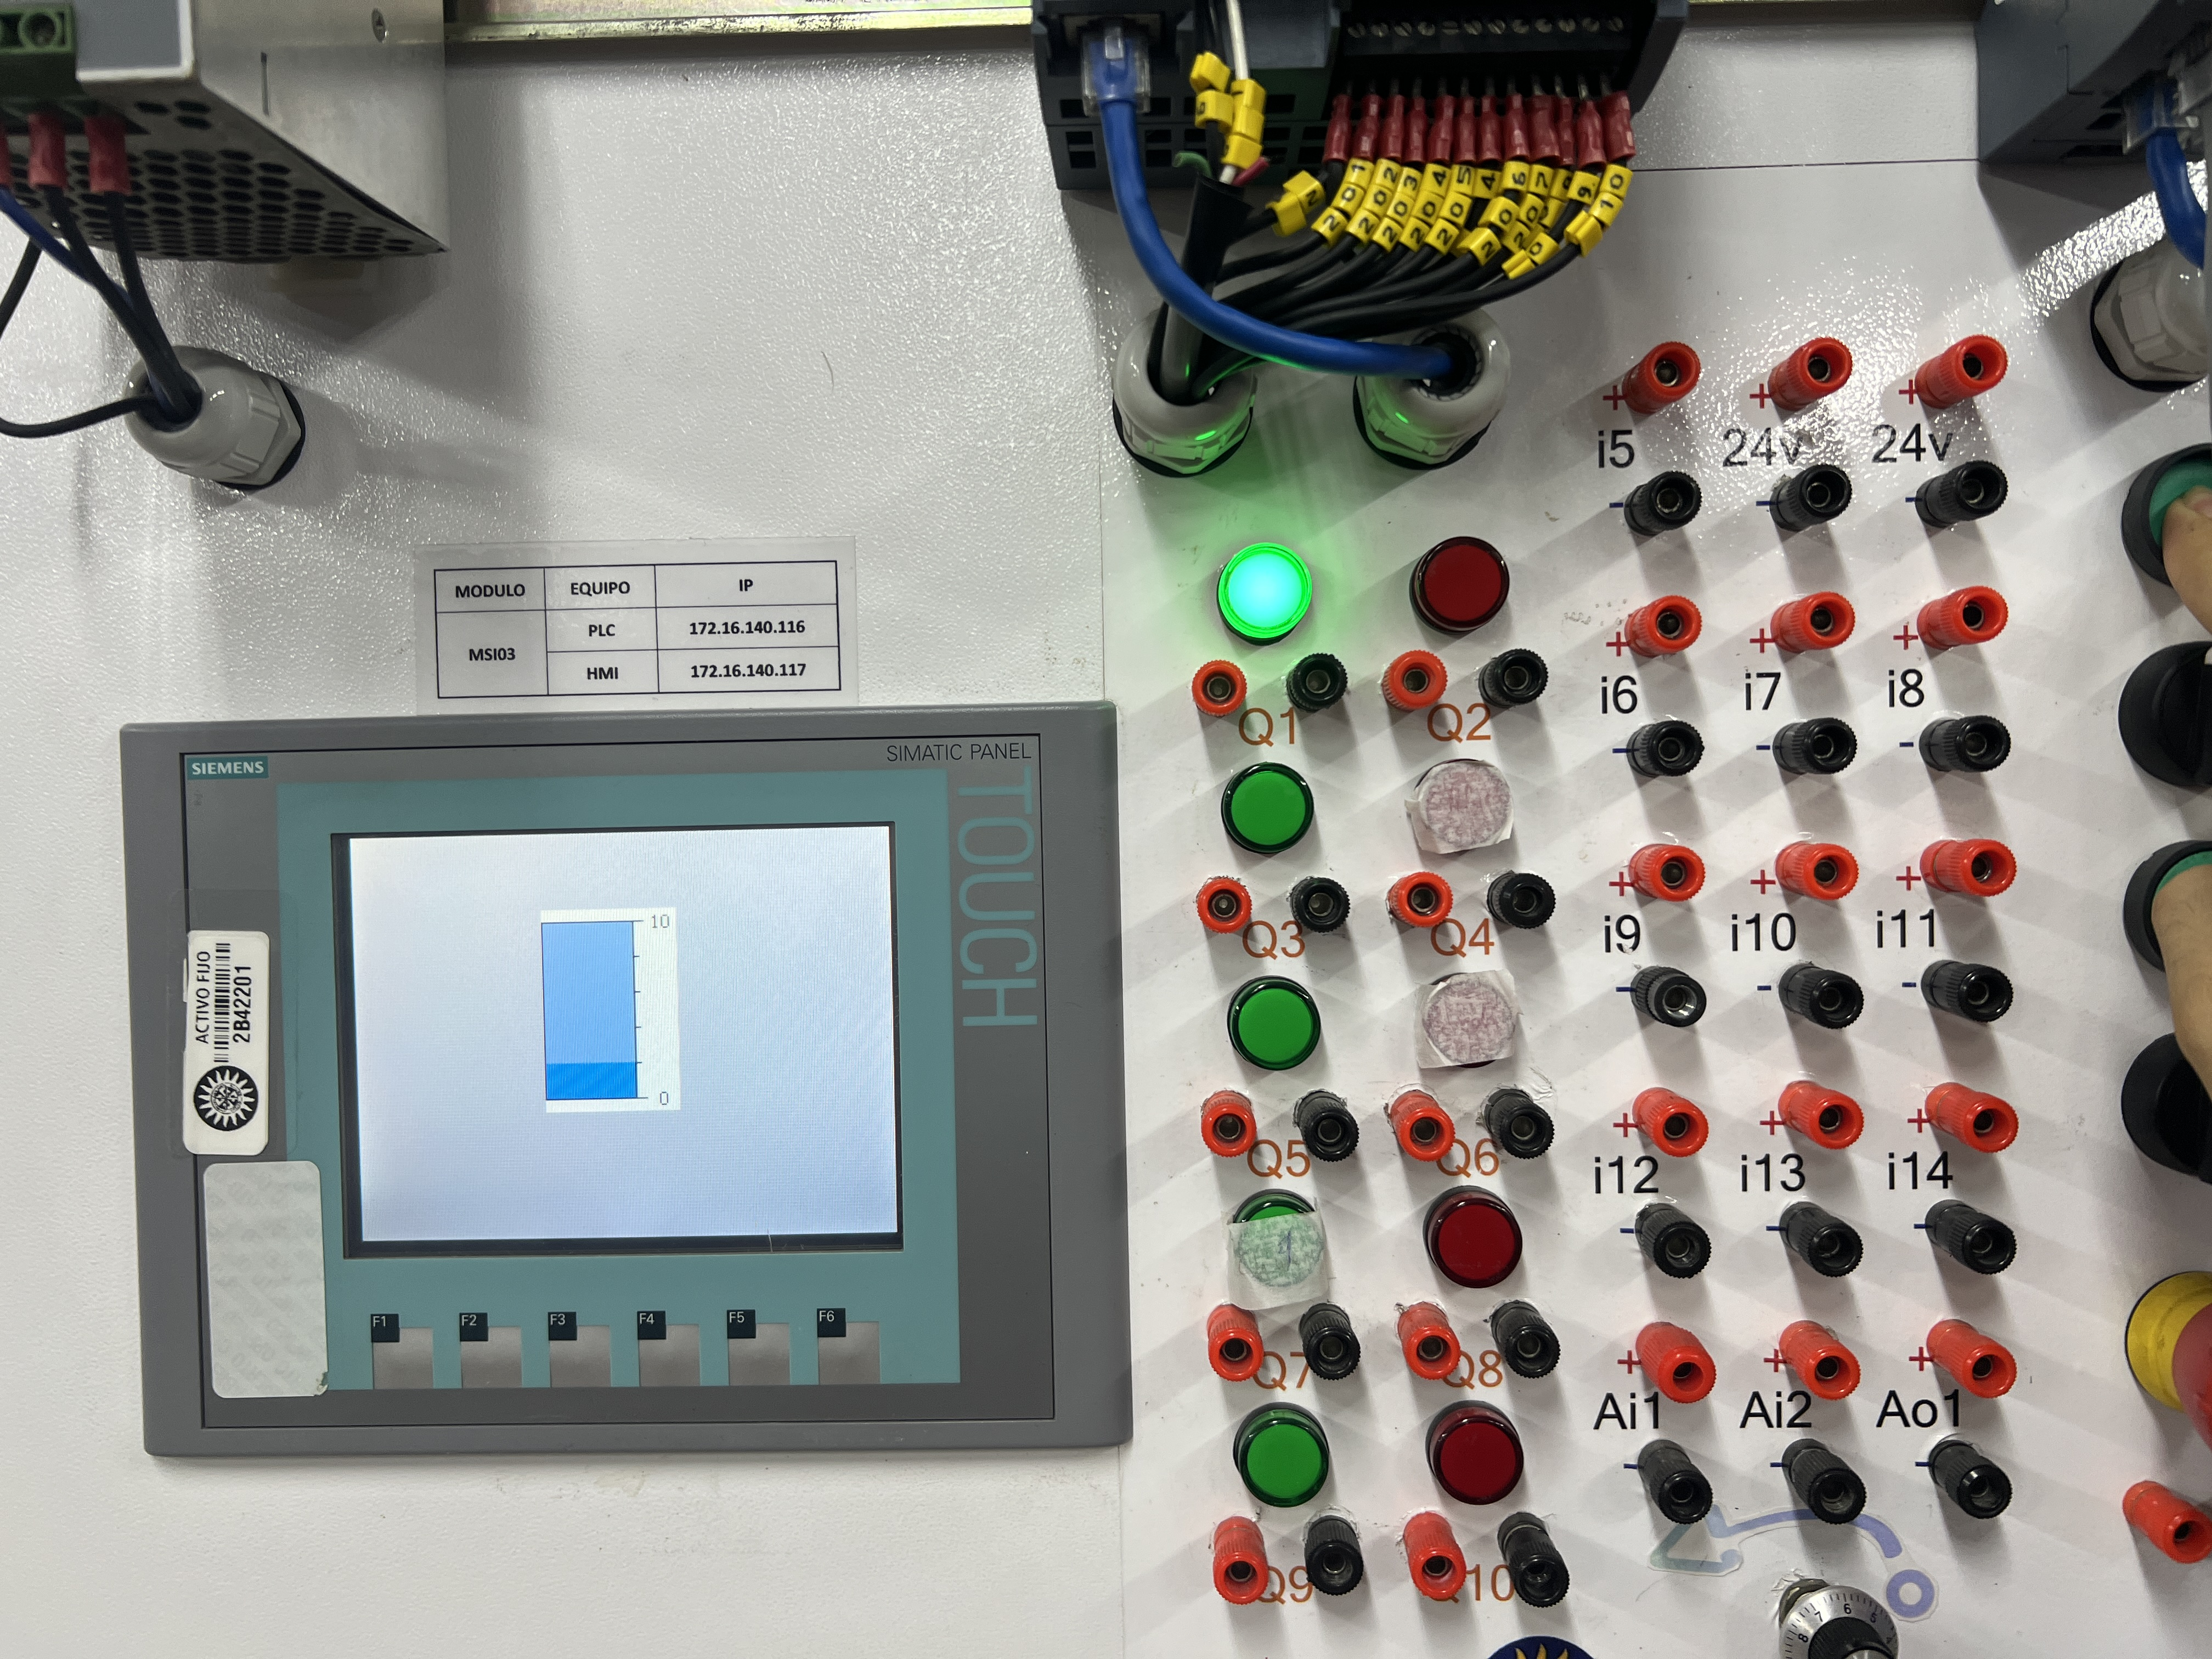
\includegraphics[width=0.4\textwidth]{figuras/HMIACCIONADO.JPG}
\caption{Accionamiento e interfaz del panel HMI.}
\label{fig:hmi_accionado}
\end{figure}

{En esta figura se observa el accionamiento del pulsador como simulación de una entrada analogica en el PLC, sacando una salida analogica en el led indicador y siendo visible dentro del HMI este cambio, como forma de simulación del volumen.}

\begin{figure}[H]
\centering
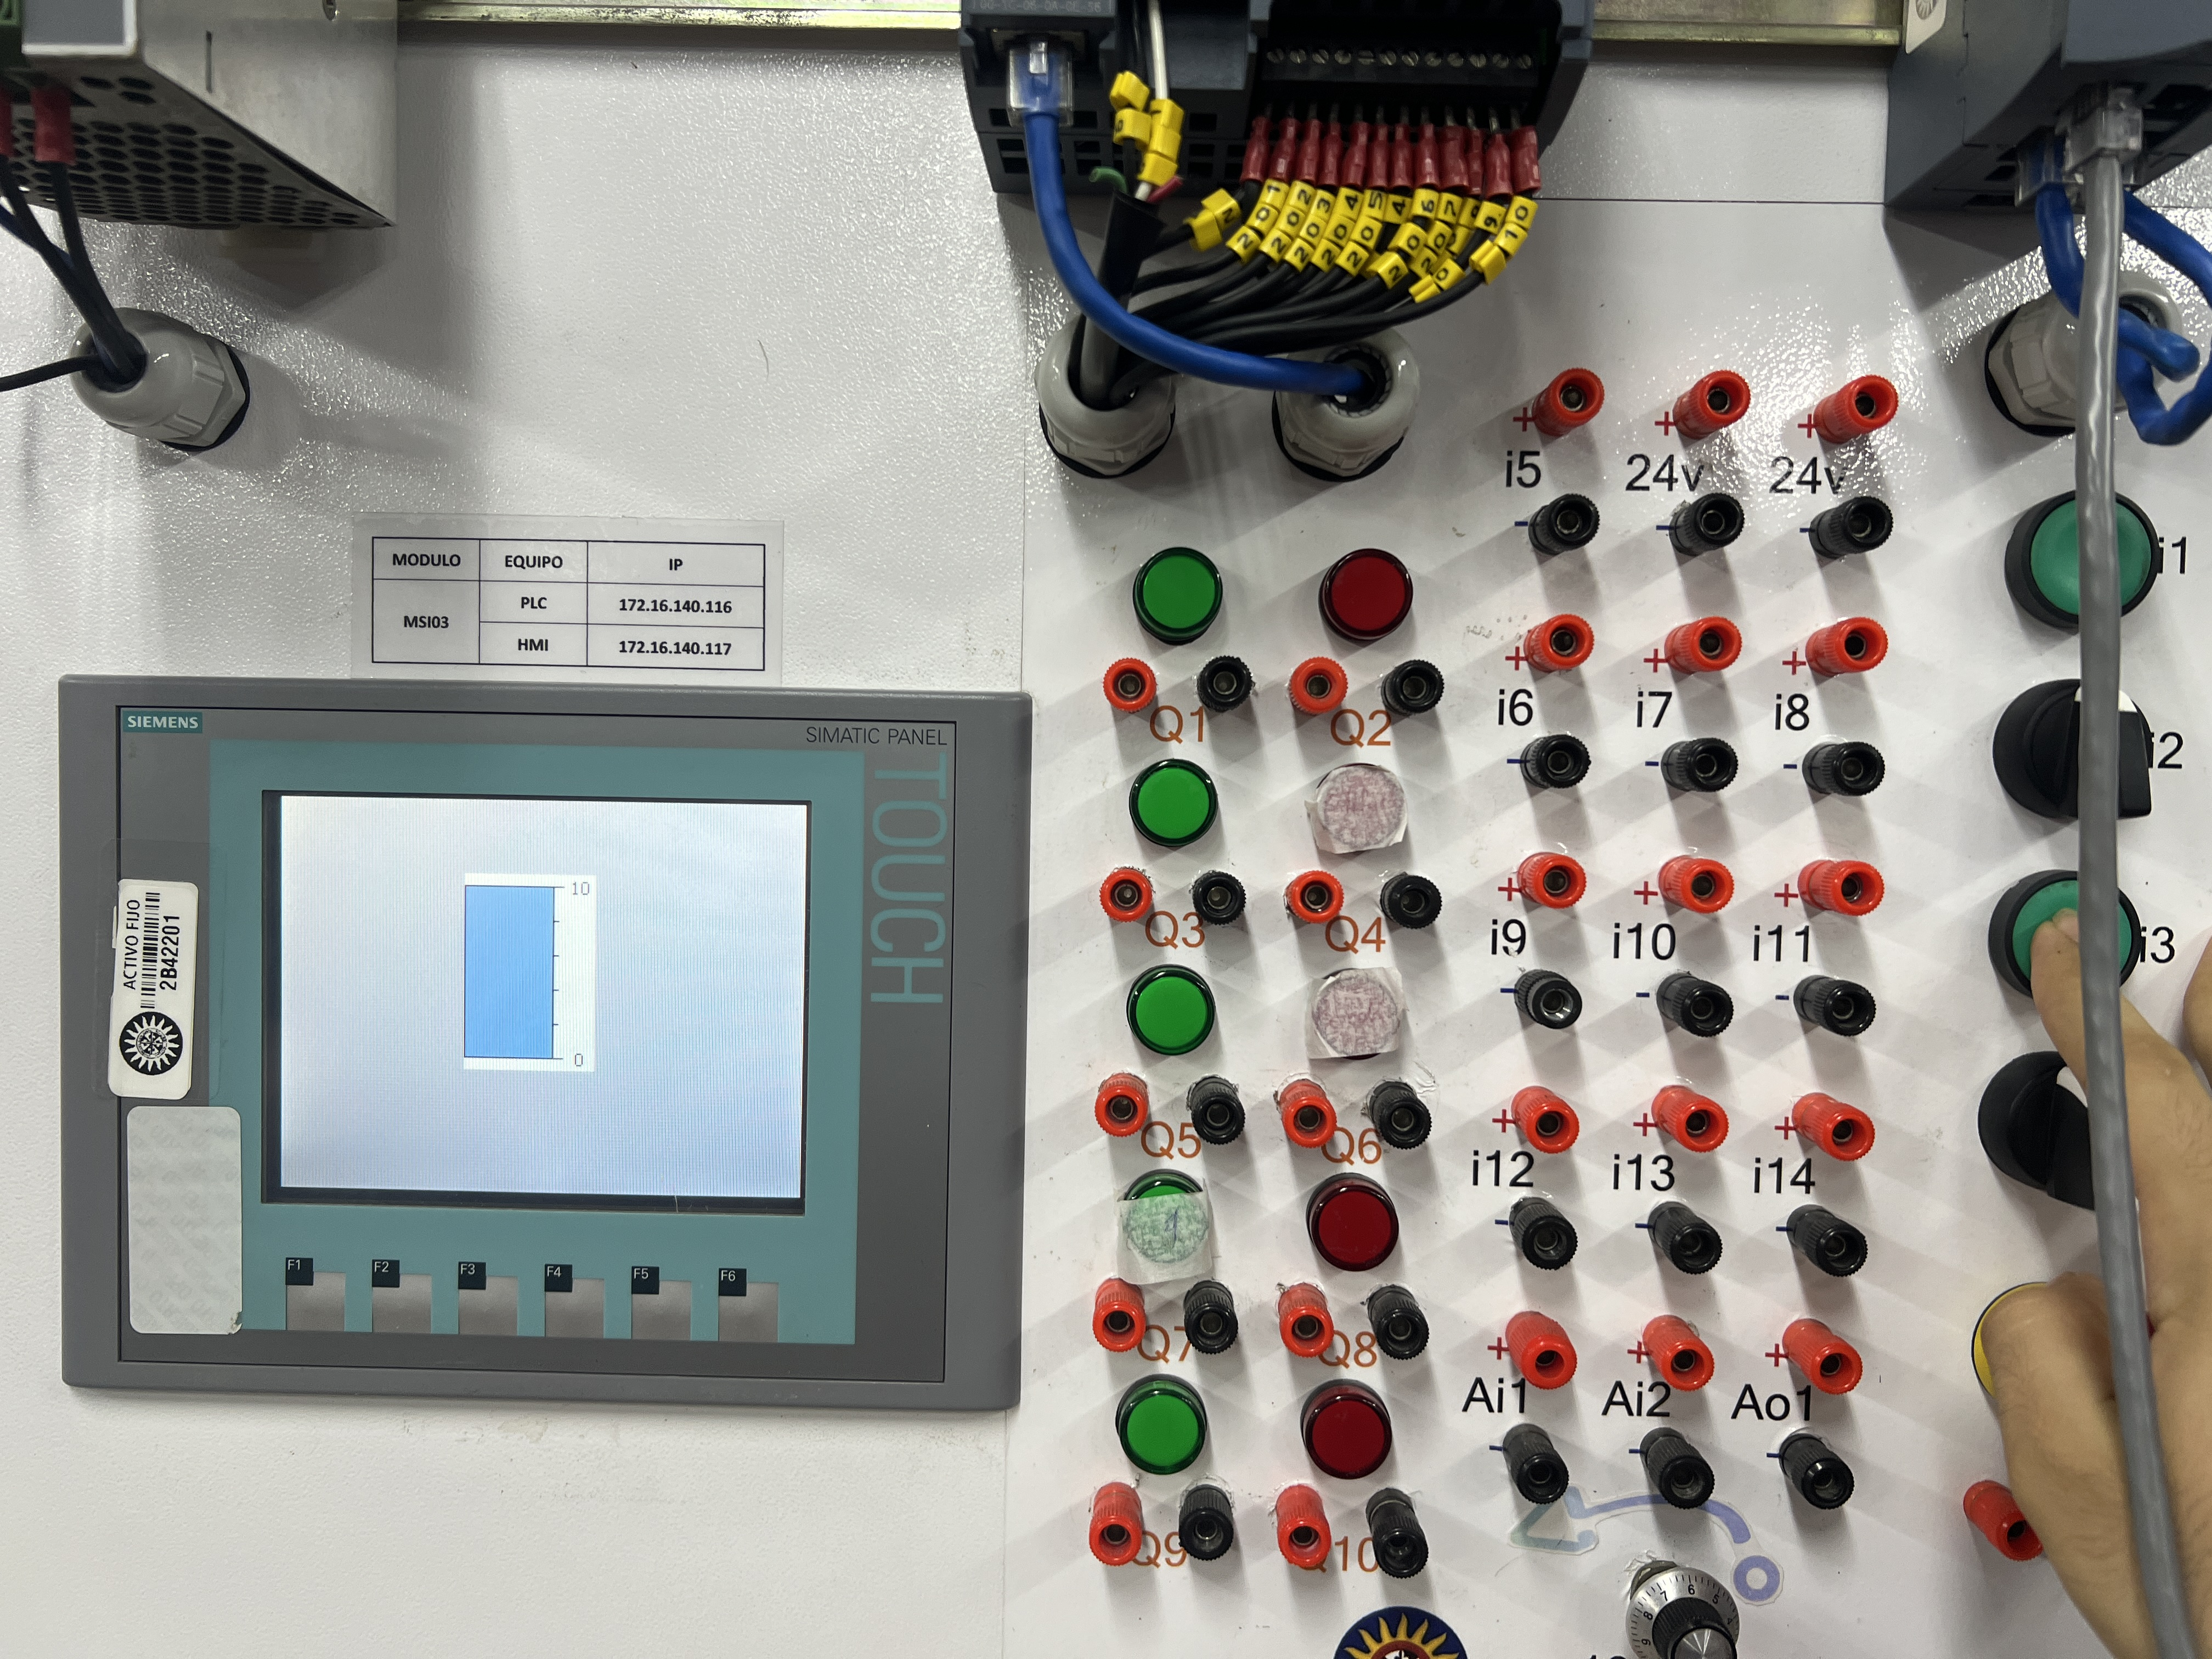
\includegraphics[width=0.7\textwidth]{figuras/RESETEARESTADO.JPG}
\caption{Reinicio y reseteo de estados del sistema.}
\label{fig:resetear_estado}
\end{figure}

{Reseteo del sistema para volver a contar desde 0, con otra entrada de pulsador, como forma de reinicio del sistema y volver a simular el llenado del tanque.}

\begin{figure}[H]
\centering
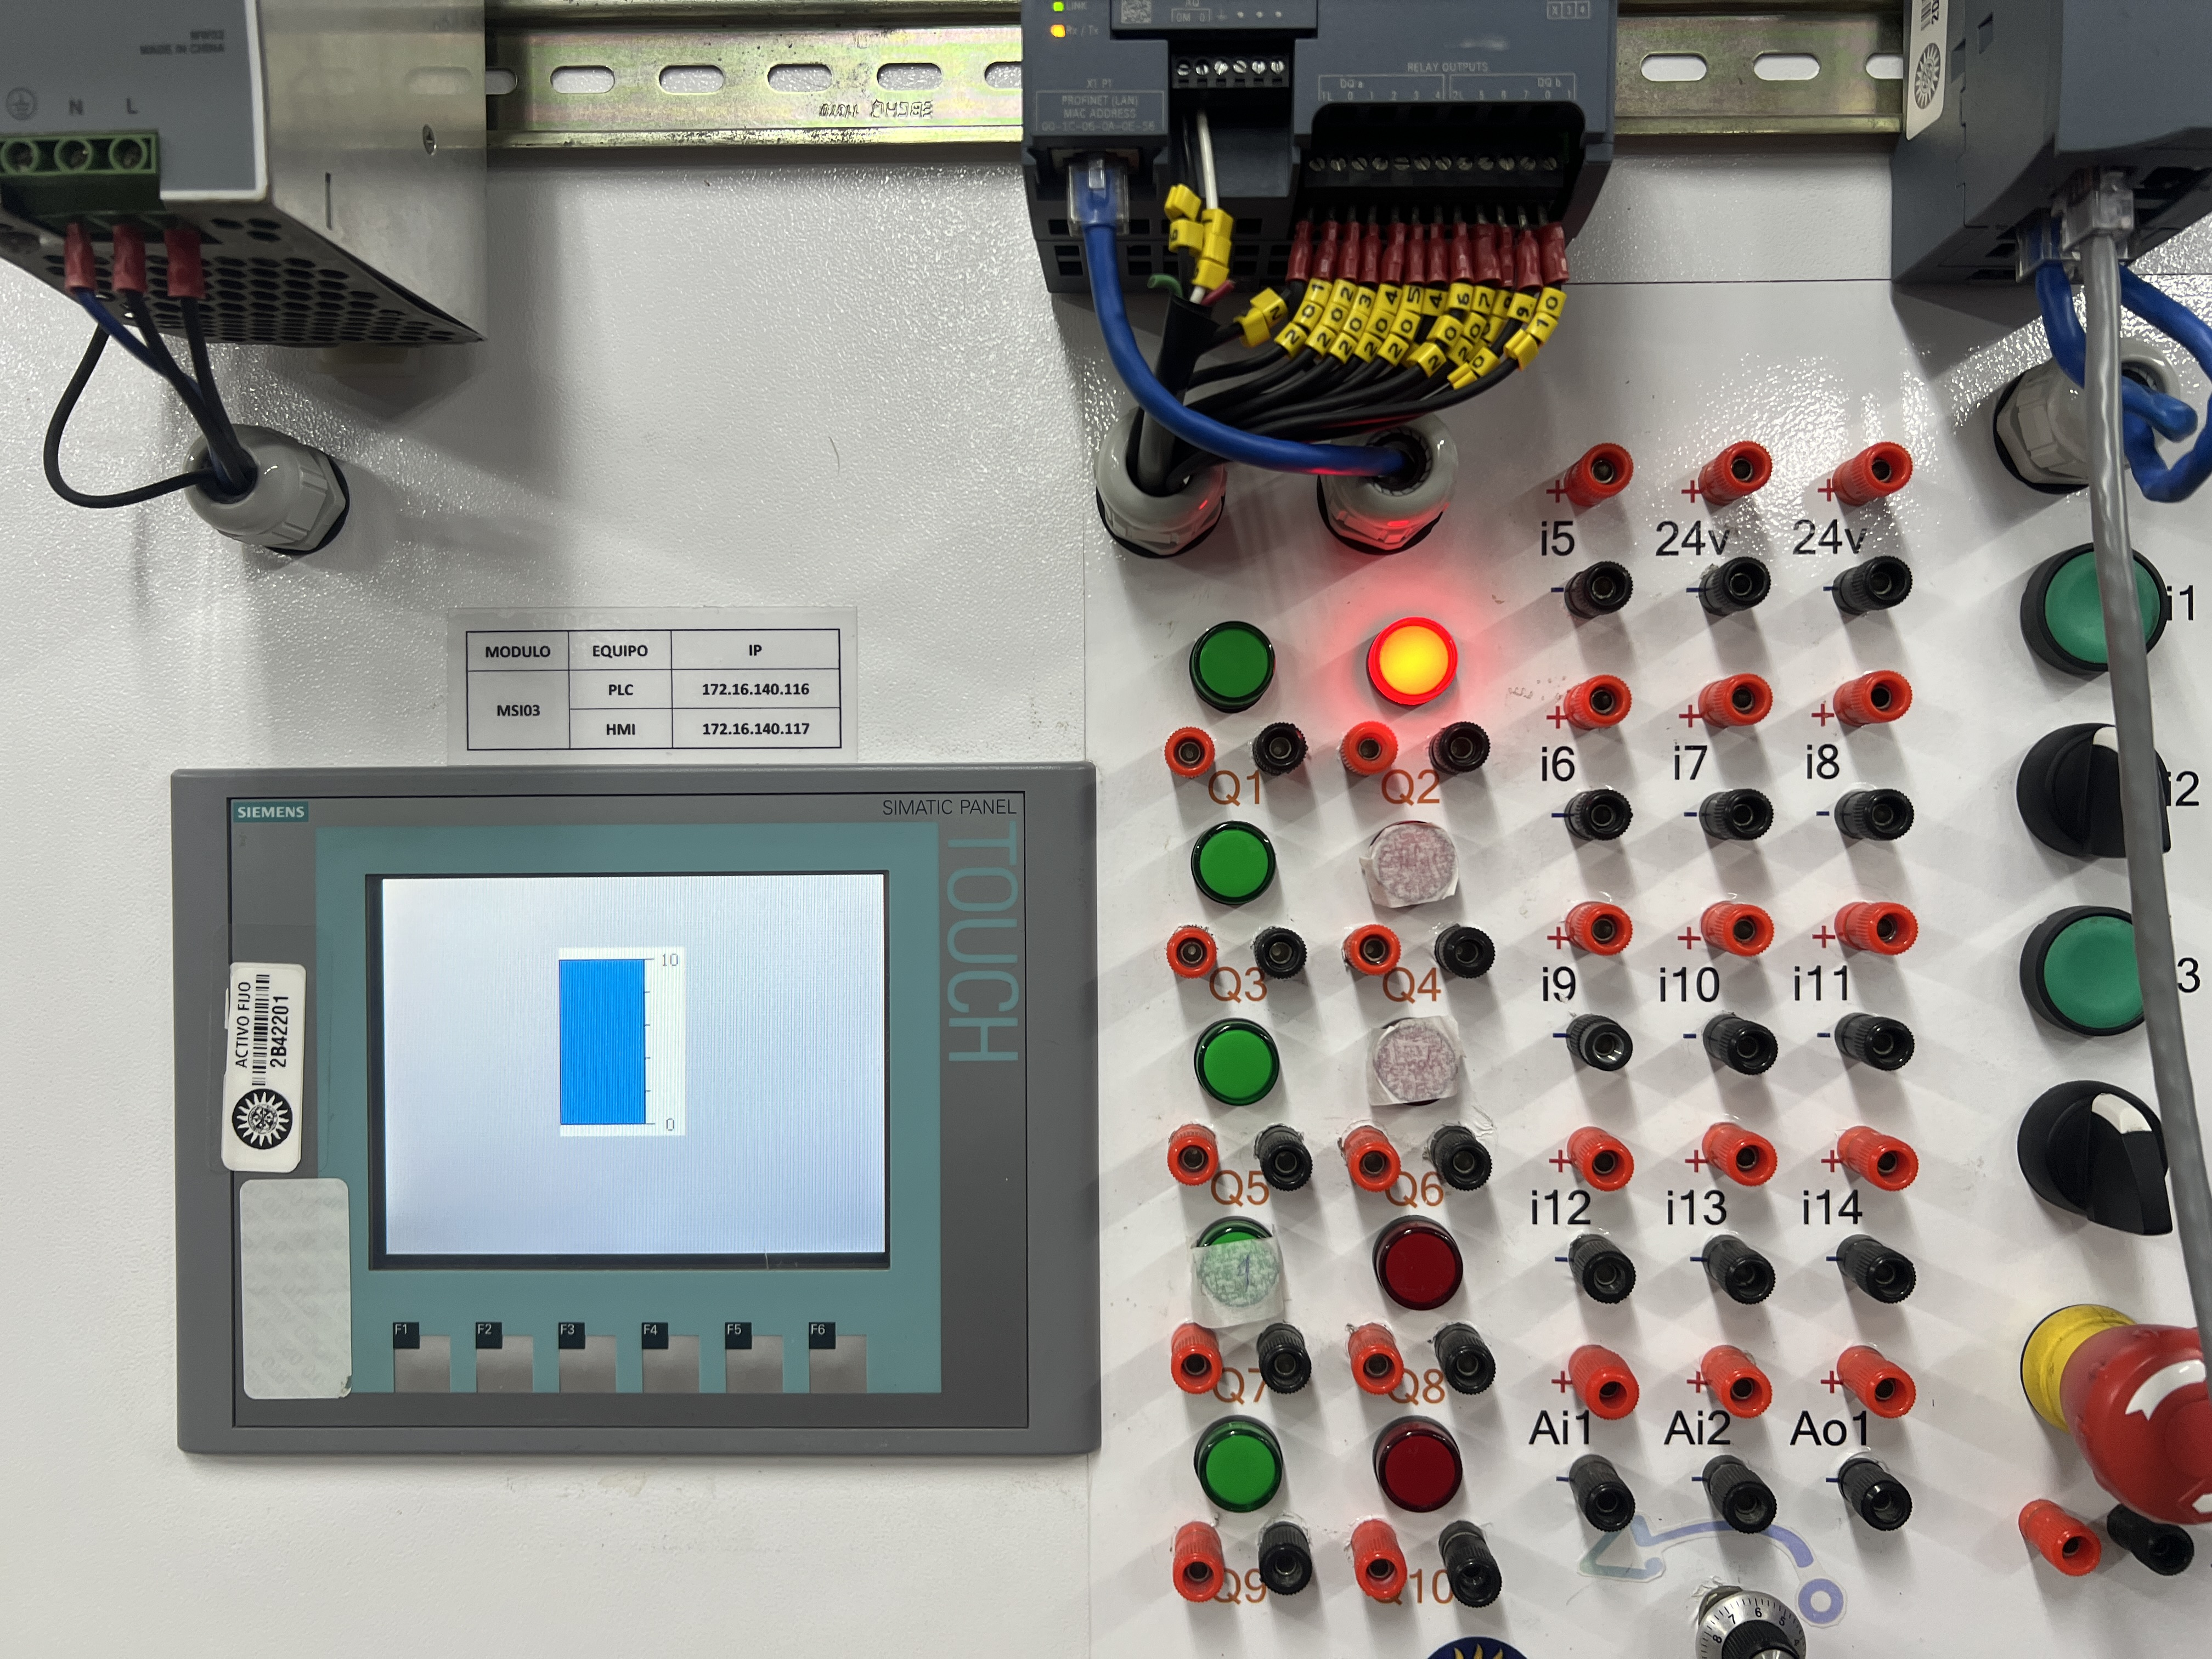
\includegraphics[width=0.7\textwidth]{figuras/SIM_TANQUE_LLENO.JPG}
\caption{Simulación de la condición de tanque lleno.}
\label{fig:sim_tanque_lleno}
\end{figure}

{Muestra la condición de tanque lleno, con la activación de la salida del led indicador y el cambio en el HMI, como forma de simulación de la condición de llenado del tanque.}

{El funcionamiento real de la programación realizada para esta simulación se puede observar en las siguientes figuras, donde se observa el código en ladder, la tabla de variables y la conexión de las variables del PLC con el HMI, verificando que existe la comunicación entre ambos equipos y que se puede visualizar el cambio de estado de las variables.}

\begin{figure}[H]
    \centering
    
\includegraphics[width=0.9\textwidth]{TABLADEVARIABLES.png}
    \caption{Nombre de las variables y su tipo asignado para la simulación.}
    \label{fig:TABLADEVARIABLES}
\end{figure}

\begin{figure}[H]
    \centering
    
\includegraphics[width=0.75\textwidth]{MAIN.png}
    \caption{Código ladder principal con el que se implementó el funcionamiento de la evidencia.}
    \label{fig:MAIN}
\end{figure}

\begin{figure}[H]
    \centering
    
\includegraphics[width=0.5\textwidth]{HMI.png}
    \caption{Impresión del HMI con las variables relacionadas.}
    \label{fig:HMI}
\end{figure}
